\documentclass[11pt,aspectratio=169]{beamer}
\usepackage[italian]{babel}
\usepackage[latin1]{inputenc}
\usepackage{graphicx}
\usepackage{listings}
\usepackage[export]{adjustbox}
% Custom bullets
\usepackage{pifont}
\usepackage[useregional]{datetime2}
\usepackage{tikz}
\usepackage[table]{colortbl}
\usepackage{venndiagram}
\usepackage{amsmath}
\usepackage{fancyvrb} % indent in verbatim


% custom legend
\newcommand{\cbox}[1]{\raisebox{\depth}{\fcolorbox{black}{#1}{\null}}}

\usetheme{Madrid}
\usecolortheme{spruce}

% Redefine labels
\deftranslation[to=Italian]{Section}{Sezione}
\deftranslation[to=Italian]{Subsection}{Sottosezione}

% Join commands
\def\ojoin{\setbox0=\hbox{$\bowtie$}%
  \rule[-.02ex]{.25em}{.4pt}\llap{\rule[\ht0]{.25em}{.4pt}}}
\def\leftouterjoin{\mathbin{\ojoin\mkern-5.8mu\bowtie}}
\def\rightouterjoin{\mathbin{\bowtie\mkern-5.8mu\ojoin}}
\def\fullouterjoin{\mathbin{\ojoin\mkern-5.8mu\bowtie\mkern-5.8mu\ojoin}}

% highlight text
\lstset{
  basicstyle=\ttfamily,
  escapeinside=||
}

\author[Gianluca Lanchini \and Piermichele Rosati]{Gianluca Lanchini \and Piermichele Rosati}

\institute[]{\large Universit\`a di Camerino\\ \footnotesize Tutorato - Basi di Dati}

\title[MySQL e MySQLWorkbench, Ancora Query]{6. MySQL e MySQLWorkbench, Ancora Query}
\subtitle{Esempio Biblioteca, Sakila DB, World DB, Esercizi Random}
\setbeamertemplate{navigation symbols}{}
\setbeamertemplate{section in toc}[sections numbered]
\setbeamertemplate{subsection in toc}[subsections numbered]
%\titlegraphic{
\includegraphics[width=6cm]{img/unicam-logo.jpg}}
\makeatletter
\setbeamertemplate{footline}{
    \leavevmode%
    \hbox{%
        \begin{beamercolorbox}[wd=.333333\paperwidth,ht=2.25ex,dp=1ex,center]{author in head/foot}%
            \usebeamerfont{author in head/foot}\insertshortauthor
        \end{beamercolorbox}%
        \begin{beamercolorbox}[wd=.333333\paperwidth,ht=2.25ex,dp=1ex,center]{title in head/foot}%
            \usebeamerfont{title in head/foot}\insertshorttitle
        \end{beamercolorbox}%
        \begin{beamercolorbox}[wd=.333333\paperwidth,ht=2.25ex,dp=1ex,right]{date in head/foot}%
            \usebeamerfont{date in head/foot}\today\hspace*{5 em}
            \insertframenumber{} / \inserttotalframenumber\hspace*{2ex} 
        \end{beamercolorbox}%
    }%
    \vskip0pt%
}
\makeatother


\AtBeginSection[]
{
\begin{frame}<beamer>
\frametitle{Indice}
\tableofcontents[currentsection]
\end{frame}
}

\begin{document}
\begin{frame}
\centering

\includegraphics[width=5.5cm]{../img/unicam-logo.jpg}
\date{\today}
\titlepage
\end{frame}
\addtobeamertemplate{frametitle}{}{%
\begin{tikzpicture}[remember picture,overlay]
\node[anchor=north east,yshift=2pt] at (current page.north east) {
\includegraphics[height=2cm]{../img/unicam-logo-notext.png}};
\end{tikzpicture}}

%\begin{frame}
%\titlepage
%\end{frame}

\section{MySQL e MySQLWorbench}
\begin{frame}{MySQL}
Il software \textbf{MySQL} \`e un sistema per la gestione di database relazionali.
\begin{columns}[T]%
    \begin{column}{0.6\textwidth}%
            \begin{itemize}[<+->]
                \item un DBMS relazionale;
                \item open-source;
                \item free;
                \item ideale per applicazioni piccole e grandi;
                \item veloce, affidabile, scalabile e facile da utilizzare;
                \item \ldots
            \end{itemize}
         \end{column}
    \begin{column}{0.4\textwidth}
        
\includegraphics[width=\textwidth]{img/logo-mysql.png}
    \end{column}
\end{columns}
\end{frame}
%
\begin{frame}{MySQLWorbench}
\textbf{MySQL Workbench} \`e uno strumento unificato di progettazione di database relazionali cross-platform e open-source che aggiunge funzionalit\`a e facilit\`a al lavoro di sviluppo di MySQL e SQL.

Caratteristiche offerte da MySQL Workbench:
    \begin{columns}[T]%
        \begin{column}{0.7\textwidth}%
                \begin{itemize}[<+->]
                    \item modellazione dei dati, lo sviluppo SQL e vari strumenti di amministrazione per la configurazione;
                    \item interfaccia grafica per lavorare con i database in modo strutturato;
                    \item creazioni di un modello grafico utilizzando MySQL Workbench.
                    \item \ldots
                \end{itemize}
             \end{column}
        \begin{column}{0.3\textwidth}
            
\includegraphics[width=.4\textwidth]{img/logo-mysql-workbench.png}
        \end{column}
    \end{columns}
\end{frame}
%
\section{Esempio: Gestione di una biblioteca}
\begin{frame}[fragile]{Creazione del database}
\begin{lstlisting}
CREATE DATABASE Biblioteca;
\end{lstlisting}
\end{frame}
%
\begin{frame}[fragile]{Utilizzo del database}
\begin{lstlisting}
USE Biblioteca;
\end{lstlisting}
\end{frame}
%
\begin{frame}[fragile]{Creazione tabella Autori}
\begin{lstlisting}
CREATE TABLE Autori (
    id_autore INT AUTO_INCREMENT PRIMARY KEY,
    nome VARCHAR(100) NOT NULL,
    cognome VARCHAR(100) NOT NULL,
    data_nascita DATE
);
\end{lstlisting}
\end{frame}
%
\begin{frame}[fragile]{Creazione tabella Libri}
\begin{lstlisting}
CREATE TABLE Libri (
    id_libro INT AUTO_INCREMENT PRIMARY KEY,
    titolo VARCHAR(255) NOT NULL,
    id_autore INT,
    genere VARCHAR(50),
    anno_pubblicazione YEAR,
    FOREIGN KEY (id_autore) REFERENCES Autori(id_autore)
);
\end{lstlisting}
\end{frame}
%
\begin{frame}[fragile]{Creazione tabella Utenti}
\begin{lstlisting}
CREATE TABLE Utenti (
    id_utente INT AUTO_INCREMENT PRIMARY KEY,
    nome VARCHAR(100) NOT NULL,
    cognome VARCHAR(100) NOT NULL,
    data_nascita DATE,
    email VARCHAR(255) UNIQUE
);
\end{lstlisting}
\end{frame}
%
\begin{frame}[fragile]{Creazione tabella Prestiti}
\begin{lstlisting}
CREATE TABLE Prestiti (
    id_prestito INT AUTO_INCREMENT PRIMARY KEY,
    id_libro INT,
    id_utente INT,
    data_prestito DATE,
    data_restituzione DATE,
    FOREIGN KEY (id_libro) REFERENCES Libri(id_libro),
    FOREIGN KEY (id_utente) REFERENCES Utenti(id_utente)
);
\end{lstlisting}
\end{frame}
%
\begin{frame}[fragile]{Popolazione tabella Autori}
\begin{lstlisting}
INSERT INTO Autori (nome, cognome, data_nascita)
VALUES 
('Luigi', 'Rossi', '1960-05-12'),
('Maria', 'Bianchi', '1975-08-23'),
('Giovanni', 'Verdi', '1980-11-15'),
('Laura', 'Neri', '1990-02-05'),
('Marco', 'Gialli', '1955-12-30');        
\end{lstlisting}
\end{frame}
%
\begin{frame}[fragile]{Popolazione tabella Libri}
\begin{lstlisting}
INSERT INTO Libri (titolo, id_autore, genere, anno_pubblicazione)
VALUES 
('Il mistero della casa abbandonata', 1, 'Giallo', 1998),
('Viaggio nel tempo', 2, 'Fantascienza', 2005),
('L\'amore ai tempi del colera', 3, 'Romanzo', 2000),
('La citta eterna', 4, 'Storico', 2010),
('Le avventure di Tom Sawyer', 5, 'Avventura', 1995);    
\end{lstlisting}
\end{frame}
%
\begin{frame}[fragile]{Popolazione tabella Utenti}
\begin{lstlisting}
INSERT INTO Utenti (nome, cognome, data_nascita, email)
VALUES 
('Anna', 'Rossi', '1992-03-17', 'anna.rossi@example.com'),
('Luca', 'Bianchi', '1988-07-12', 'luca.bianchi@example.com'),
('Chiara', 'Verdi', '1995-11-29', 'chiara.verdi@example.com'),
('Giorgio', 'Neri', '1983-05-08', 'giorgio.neri@example.com'),
('Sara', 'Gialli', '2000-01-20', 'sara.gialli@example.com');
\end{lstlisting}
\end{frame}
%
\begin{frame}[fragile]{Popolazione tabella Prestiti}    
\begin{lstlisting}
INSERT INTO Prestiti
(id_libro, id_utente, data_prestito, data_restituzione)
VALUES 
(1, 1, '2024-01-10', '2024-01-24'),
(2, 2, '2024-02-14', '2024-02-28'),
(3, 3, '2024-03-01', '2024-03-15'),
(4, 4, '2024-04-20', '2024-05-04'),
(5, 5, '2024-05-25', '2024-06-08');    
\end{lstlisting}
\end{frame}
%
\section{Esercizi DB: Sakila}
\begin{frame}[fragile]{Schema del database Sakila}
\begin{figure}
    \centering
        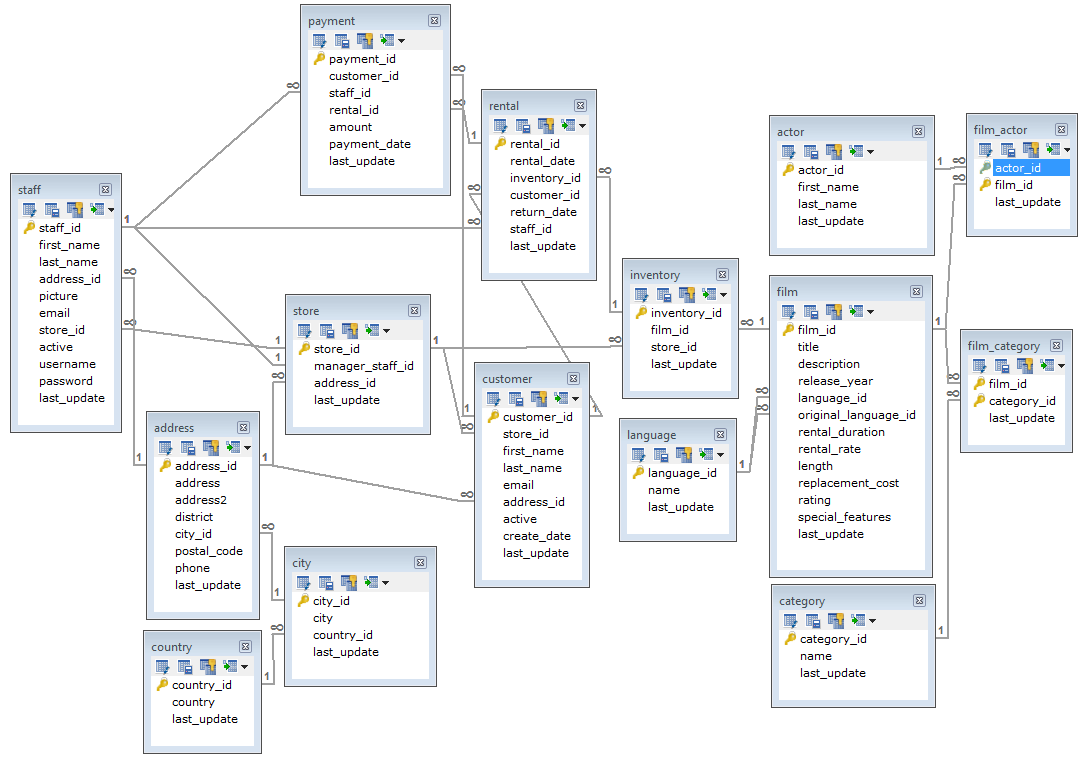
\includegraphics[width=.65\textwidth]{img/db-sakila.png}
    \end{figure}
\end{frame}
%
\begin{frame}[fragile]{Sakila: Es. 1}
Quali attori hanno il nome `Scarlett'?
\pause
\begin{lstlisting}
SELECT *
FROM actor
WHERE first_name = `Scarlett';
\end{lstlisting}
\end{frame}
%
\begin{frame}[fragile]{Sakila: Es. 2}
Quali attori hanno il cognome `Johansson'?
\pause
\begin{lstlisting}
SELECT *
FROM actor
WHERE last_name LIKE `Johansson';
\end{lstlisting}
\pause
oppure
\begin{lstlisting}
SELECT *
FROM actor
WHERE last_name = `Johansson';
\end{lstlisting}
\end{frame}
%
\begin{frame}[fragile]{Sakila: Es. 3}
Quanti cognomi distinti di attori ci sono?
\pause
\begin{lstlisting}
SELECT COUNT(DISTINCT last_name)
FROM actor;
\end{lstlisting}
\end{frame}
%
\begin{frame}[fragile]{Sakila: Es. 4}
Quali cognomi non si ripetono?
\pause
\begin{lstlisting}
SELECT last_name
FROM actor
GROUP BY last_name
HAVING COUNT(*) = 1;
\end{lstlisting}
\end{frame}
%
\begin{frame}[fragile]{Sakila: Es. 5}
Quali cognomi compaiono pi\`u di una volta?
\pause
\begin{lstlisting}
SELECT last_name
FROM actor
GROUP BY last_name
HAVING COUNT(*) > 1;
\end{lstlisting}
\end{frame}
%
\begin{frame}[fragile]{Sakila: Es. 6}
Qual \`e l'attore che ha recitato nel maggior numero di film?
\pause
\begin{lstlisting}
SELECT actor.actor_id, actor.first_name, actor.last_name,
COUNT(actor.actor_id) AS film_count
FROM actor JOIN film_actor
ON actor.actor_id = film_actor.actor_id
GROUP BY film_actor.actor_id
ORDER BY film_count DESC
LIMIT 1;
\end{lstlisting}
\end{frame}
%
\begin{frame}[fragile]{Sakila: Es. 7}
Inserire un record per rappresentare `Mary Smith' che oggi affitta `Academy Dinosaur' da `Mike Hillyer' presso lo Store 1.
\pause
\newline
\newline
Per ottenere la data ed orario corrente: '\textbf{NOW()}'
\end{frame}

\begin{frame}[fragile]{Sakila: Es. 7}
Inserire un record per rappresentare `Mary Smith' che oggi affitta `Academy Dinosaur' da `Mike Hillyer' presso lo Store 1.
\newline
\newline
Per ottenere l'id dell'articolo 'Academy Dinosaur':
\begin{lstlisting}
SELECT inv.inventory_id
FROM inventory AS inv
JOIN film AS fi ON inv.film_id = fi.film_id
WHERE fi.title = 'Academy Dinosaur'
AND inv.store_id = 1
LIMIT 1;
\end{lstlisting}
\end{frame}

\begin{frame}[fragile]{Sakila: Es. 7}
Inserire un record per rappresentare `Mary Smith' che oggi affitta `Academy Dinosaur' da `Mike Hillyer' presso lo Store 1.
\newline
\newline
Per ottenere l'id del cliente 'Mary Smith':
\begin{lstlisting}
SELECT customer_id
FROM customer
WHERE first_name = 'Mary' AND last_name = 'Smith'
AND store_id = 1;
\end{lstlisting}
\end{frame}

\begin{frame}[fragile]{Sakila: Es. 7}
Inserire un record per rappresentare `Mary Smith' che oggi affitta `Academy Dinosaur' da `Mike Hillyer' presso lo Store 1.
\newline
\newline
Per ottenere l'id del commesso 'Mike Hillyer':
\begin{lstlisting}
SELECT staff_id
FROM staff
WHERE first_name = 'Mike' AND last_name = 'Hillyer'
AND store_id = 1;
\end{lstlisting}
\end{frame}

\begin{frame}[fragile]{Sakila: Es. 7}
Inserire un record per rappresentare `Mary Smith' che oggi affitta `Academy Dinosaur' da `Mike Hillyer' presso lo Store 1.
\begin{lstlisting}
INSERT INTO rental
(rental_date, inventory_id, customer_id, staff_id)
VALUES
(NOW(), 1, 1, 1);
\end{lstlisting}
\end{frame}

%
\begin{frame}[fragile]{Sakila: Es. 8}
Qual \`e la lunghezza media di tutti i film del DB sakila?
\pause
\begin{lstlisting}
SELECT AVG(length)
FROM film;
\end{lstlisting}
\end{frame}
%
\begin{frame}[fragile]{Sakila: Es. 9}
Qual \`e la durata media dei film per categoria?
\pause
\begin{lstlisting}
SELECT category.name, AVG(length)
FROM film JOIN film_category
ON film.film_id = film_category.film_id
JOIN category
ON film_category.category_id = category.category_id
GROUP BY category.category_id
ORDER BY AVG(length) DESC;
\end{lstlisting}
\end{frame}
%
\begin{frame}[fragile]{Sakila: Es. 10}
Elenco i titoli di tutti i film che durano pi\`u di 113 minuti:
\pause
\begin{lstlisting}
SELECT title
FROM film
WHERE length >= 113;
\end{lstlisting}
\end{frame}
%
\begin{frame}[fragile]{Sakila: Es. 11}
Elencare i film la cui durata \`e compresa tra 130 e 150 minuti (estremi compresi) e il cui rating \`e NC-17:
\pause
\begin{lstlisting}
SELECT title
FROM film
WHERE length >=130 AND length <= 150 AND rating = `NC-17';
\end{lstlisting}
\pause
oppure
\begin{lstlisting}
SELECT title
FROM film
WHERE length BETWEEN 130 AND 150 AND rating = `NC-17';
\end{lstlisting}
\end{frame}
%
\begin{frame}[fragile]{Sakila: Es. 12}
Elencare nome e cognome di tutti gli attori che hanno recitato nel film ``TEEN APOLLO''.
\pause
\begin{lstlisting}
SELECT first_name, last_name FROM film, actor, film_actor
WHERE film.film_id = film_actor.film_id
AND actor.actor_id = film_actor.actor_id
AND film.title = `TEEN APOLLO';
\end{lstlisting}
\pause
oppure
\begin{lstlisting}
SELECT first_name, last_name
FROM film JOIN film_actor ON film.film_id = film_actor.film_id
JOIN actor ON actor.actor_id = film_actor.actor_id
AND film.title = `TEEN APOLLO';
\end{lstlisting}
\end{frame}
%
\begin{frame}[fragile]{Sakila: Es. 13}
\vspace{.5cm}
Indicare il numero di film e la durata media dei film in cui ha recitato ZERO CAGE.
\pause
\begin{lstlisting}
SELECT COUNT(*) AS `n. film' , AVG(length) AS `durata media'
FROM film JOIN film_actor
ON film.film_id = film_actor.film_id 
JOIN actor ON actor.actor_id = film_actor.actor_id
WHERE actor.first_name = `ZERO' AND actor.last_name=`CAGE';
\end{lstlisting}
\end{frame}
%
\begin{frame}[fragile]{Sakila: Es. 14}
Elencare gli attori per nome, cognome e numero di film fatti, ordinati da chi ha fatto pi\`u film a chi ne ha fatti meno e in caso di ugual numero di film ordinarli per cognome.

Nell'elenco devono comparire solo gli attori che hanno fatto pi\`u di 33 film (33 compreso).
\pause
\begin{lstlisting}
SELECT first_name, last_name, count(*) AS numero_film
FROM film JOIN film_actor
ON film.film_id = film_actor.film_id 
JOIN actor ON actor.actor_id = film_actor.actor_id
GROUP BY actor.actor_id
HAVING numero_film >= 33
ORDER BY numero_film DESC, last_name;
\end{lstlisting}
\end{frame}
%
\begin{frame}[fragile]{Sakila: Es. 15}
Trovare il film con la durata maggiore, indicandone titolo e durata.

Se fossero pi\`u di uno, elencarli in ordine di titolo.
\pause
\begin{lstlisting}
SELECT title, length
FROM film
WHERE length = (
    SELECT MAX(length)
    FROM film
    )
ORDER BY title;
\end{lstlisting}
\end{frame}
%
\begin{frame}[fragile]{Sakila: Es. 16}
Trovare quanti sono i film la cui durata \`e maggiore di almeno 60 minuti della durata media di tutti i film.
\pause
\begin{lstlisting}
SELECT COUNT(*) AS `n. film'
FROM film
WHERE length > (
    SELECT AVG(length) + 60
    FROM film
);
\end{lstlisting}
\end{frame}
%
%
\section{Esercizi DB: World}
\begin{frame}[fragile]{Schema del database World}
\begin{figure}
    \centering
        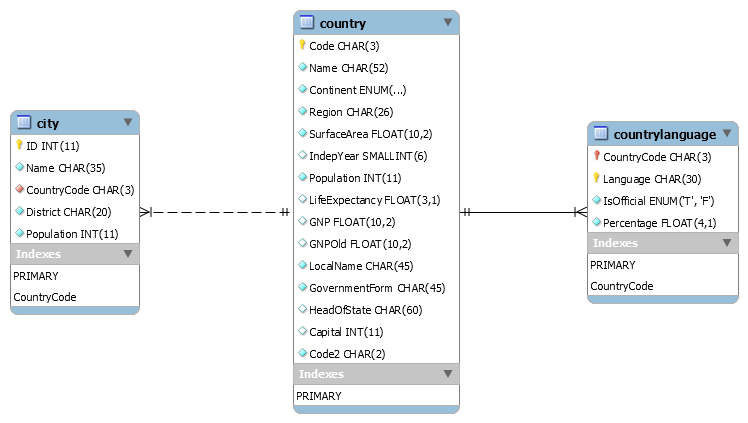
\includegraphics[width=.8\textwidth]{img/db-world.png}
    \end{figure}
\end{frame}
%
\begin{frame}[fragile]{World: Es. 1}
Visualizzare id, nome, popolazione dalla tabella \textit{city} e limitare i risultati solo alle prime 10 righe.
\pause
\begin{lstlisting}
SELECT Id, Name, Population
FROM city
LIMIT 10;
\end{lstlisting}
\end{frame}
%
\begin{frame}[fragile]{World: Es. 2}
Visualizzare id, nome, popolazione dalla tabella \textit{city} e limitare i risultati alle righe 31-40.
\pause
\begin{lstlisting}
SELECT Id, Name, Population
FROM city
LIMIT 30, 10;
\end{lstlisting}
\end{frame}
%
\begin{frame}[fragile]{World: Es. 3}
Trovare dalla tabella \textit{city} solo le citt\`a la cui popolazione \`e superiore a 2000000.
\pause
\begin{lstlisting}
SELECT Name, Population
FROM city
WHERE Population > 2000000;
\end{lstlisting}
\end{frame}
%
\begin{frame}[fragile]{World: Es. 4}
Trovare tutti i nomi di citt\`a dalla tabella \textit{city} il cui nome inizia con il prefisso ``Be''.
\pause
\begin{lstlisting}
SELECT Name
FROM city
WHERE Name LIKE `Be%';
\end{lstlisting}
\end{frame}
%
\begin{frame}[fragile]{World: Es. 5}
Trovare dalla tabella \textit{city} solo le citt\`a la cui popolazione \`e compresa tra 500000 e 1000000.
\pause
\begin{lstlisting}
SELECT Name, Population
FROM city
WHERE Population BETWEEN 500000 AND 1000000;
\end{lstlisting}
\pause
oppure
\begin{lstlisting}
SELECT Name, Population
FROM city
WHERE Population >= 500000 AND Population <=1000000;
\end{lstlisting}
\end{frame}
%
\begin{frame}[fragile]{World: Es. 6}
Visualizzare tutte le citt\`a della tabella \textit{city} ordinate per nome in ordine crescente.
\pause
\begin{lstlisting}
SELECT *
FROM city
ORDER BY Name ASC;
\end{lstlisting}
oppure
\pause
\begin{lstlisting}
SELECT *
FROM city
ORDER BY Name;
\end{lstlisting}
\end{frame}
%
\begin{frame}[fragile]{World: Es. 7}
Trovare la citt\`a con la popolazione pi\`u bassa nella tabella \textit{city}.
\pause
\vspace{-.1cm}
\begin{lstlisting}
SELECT Population, Name
FROM city
WHERE Population IS NOT NULL
ORDER BY Population ASC
LIMIT 1;
\end{lstlisting}
\end{frame}
%
\begin{frame}[fragile]{World: Es. 7}
Trovare la citt\`a con la popolazione pi\`u bassa nella tabella \textit{city}.

Altra possibile soluzione:
\vspace{-.1cm}
\begin{lstlisting}
SELECT MIN(Population), Name
FROM city
GROUP BY Name,Population
HAVING MIN(Population) ORDER BY Population
LIMIT 1;
\end{lstlisting}
\end{frame}
%
\begin{frame}[fragile]{World: Es. 8}
Trovare la citt\`a con la popolazione pi\`u bassa nella tabella \textit{country}.
\\Altra possibile soluzione:
\pause
\\Prima troviamo la \textbf{popolazione pi\`u bassa}:
\begin{lstlisting}
SELECT MIN(Population)
FROM country;
\end{lstlisting}
\pause
Poi facciamo una \textbf{query annidata} dove cerchiamo tutte le citt\`a che hanno poplazione = a quella appena trovata:
\begin{lstlisting}
SELECT Name, Population
FROM country
WHERE Population = (
    SELECT MIN(Population)
    FROM country
);
\end{lstlisting}
\end{frame}
%
\begin{frame}[fragile]{World: Es. 9}
Trovare il paese con la popolazione pi\`u numerosa nella tabella \textit{country}.
\pause
\begin{lstlisting}
SELECT Population, Name
FROM country
WHERE Population IS NOT NULL
ORDER BY Population DESC
LIMIT 1;
\end{lstlisting}
\end{frame}
%
\begin{frame}[fragile]{World: Es. 9}
Trovare il paese con la popolazione pi\`u numerosa nella tabella \textit{country}.

Altra soluzione possibile:
\pause
\\Prima troviamo la \textbf{pi\`u alta aspettativa di vita}:
\begin{lstlisting}
SELECT MAX(Population)
FROM country;
\end{lstlisting}
\pause
Poi facciamo una \textbf{query annidata} dove cerchiamo tutte le citt\`a che hanno come popolazione quella appena trovata:
\begin{lstlisting}
SELECT Population, Name
FROM country
WHERE Population = (
    SELECT MAX(Population)
    FROM country
);
\end{lstlisting}
\end{frame}
%
\begin{frame}[fragile]{World: Es. 10}
Elencare tutte le lingue parlate nella regione dei Caraibi (``Caribbean''). 
\pause
\begin{lstlisting}
SELECT country.Region, countrylanguage.Language
FROM country LEFT JOIN countrylanguage
ON country.Code = countrylanguage.CountryCode
WHERE country.Region = ``Caribbean'';
\end{lstlisting}
\end{frame}
%
\begin{frame}[fragile]{World: Es. 11}
Trovare la capitale della Spagna (ESP).
\pause
\begin{lstlisting}
SELECT city.Name
FROM city JOIN country ON city.ID = country.Capital
WHERE city.CountryCode = `ESP';
\end{lstlisting}
\end{frame}
%
\begin{frame}[fragile]{World: Es. 12}
Trovare il paese con la pi\`u alta aspettativa di vita.
\pause
\begin{lstlisting}
SELECT country.Name, LifeExpectancy
FROM country
ORDER BY LifeExpectancy DESC
LIMIT 1;
\end{lstlisting}
\end{frame}
%
\begin{frame}[fragile]{World: Es. 12}
Trovare il paese con la pi\`u alta aspettativa di vita.

Altra soluzione Possibile:
\pause
\\Prima troviamo la \textbf{pi\`u alta aspettativa di vita}:
\begin{lstlisting}
SELECT MAX(LifeExpectancy)
FROM country;
\end{lstlisting}
\pause
Poi facciamo una \textbf{query annidata} dove cerchiamo quell'aspettativa di vita appena trovata:
\begin{lstlisting}
SELECT country.Name, LifeExpectancy
FROM country
WHERE LifeExpectancy = (
    SELECT MAX(LifeExpectancy)
    FROM country
);
\end{lstlisting}
\end{frame}
%
\begin{frame}[fragile]{World: Es. 13}
Trovare tutte le citt\`a del continente europeo.
\pause
\begin{lstlisting}
SELECT city.Name
FROM city JOIN country ON city.CountryCode = country.Code
WHERE country.Continent = `Europe';
\end{lstlisting}
\end{frame}
%
\begin{frame}[fragile]{World: Es. 14}
Aggiornare il presidente degli Stati Uniti attualmente presente sul database, con `Donald Trump'.
\pause
\begin{lstlisting}
UPDATE country
SET HeadOfState = `Donald Trump'
WHERE Name = `United States';
\end{lstlisting}
\end{frame}
%
\begin{frame}[fragile]{World: Es. 15}
Trovare la citt\`a pi\`u popolata nella tabella \textit{city}.
\pause
\newline
\\Stesso ragionamento delle query precedenti (query annidata):
\begin{lstlisting}
SELECT Name, Population
FROM city
WHERE Population = (
    SELECT MAX(Population)
    FROM city
);
\end{lstlisting}
\end{frame}
%
\begin{frame}[fragile]{World: Es. 16}
Trovare la citt\`a meno popolata nella tabella \textit{city}.
\pause
\newline
\\Stesso ragionamento delle query precedenti (query annidata):
\begin{lstlisting}
SELECT Name, Population
FROM city
WHERE Population = (
    SELECT MIN(Population)
    FROM city
);
\end{lstlisting}
\end{frame}
%
\begin{frame}[fragile]{World: Es. 17}
Calcolare il numero di record della tabella \textit{city}.
\pause
\begin{lstlisting}
SELECT COUNT(Id) AS `n. di citta'
FROM city;
\end{lstlisting}
\end{frame}
%
\begin{frame}[fragile]{World: Es. 18}
Ottenere il numero di citt\`a in Cina dalla tabella \textit{city}.

La Cina ha country code ``CHN''.
\pause
\begin{lstlisting}
SELECT COUNT(*)
FROM city
WHERE CountryCode = ``CHN'';
\end{lstlisting}
\end{frame}
%
%
\section{Esercizi Random}
\def\schemaPersonaMatrimonio{\small \begin{align*}
    &PERSONA(\underline{CF}, cognome, nome, annoNascita, sesso)\\
    &MATRIMONIO(\underline{CFmoglie}, \underline{CFmarito}, anno, luogo)
    \end{align*}}
\def\schemaNegoziProdottiListino{\small \begin{align*}
    &NEGOZI(\underline{IDnegozio}, nome, citta)\\
    &PRODOTTI(\underline{codProdotto}, nomeProdotto, marca)\\
    &LISTINO(\underline{negozio}, \underline{prodotto}, prezzo)
    \end{align*}}
\def\schemaVenditeClientiDettagliVendite{\small \begin{align*}
    &Vendite(\underline{NumeroScontrino}, Data)\\
    &Clienti(\underline{Codice}, Cognome, Eta)\\
    &DettagliVendite(\underline{NumeroScontrino}, \underline{Riga}, Prodotto, Importo, Cliente)
    \end{align*}}
\def\schemaClientiNoleggiAuto{\small \begin{align*}
    &CLIENTI(\underline{Codice}, Nome, Indirizzo, Citta)\\
    &NOLEGGI(\underline{Cliente}, \underline{Auto}, DataPrelievo, DataRestituzione)\\
    &AUTOVETTURE(\underline{Targa}, Modello, Colore, AnnoImmatricolazione, CostoGiornaliero)
    \end{align*}}
\def\schemaProdottiVendite{\small \begin{align*}
    &PRODOTTI(\underline{Codice}, Descrizione, Marca)\\
    &VENDITE(\underline{Prodotto}, \underline{Mese}, \underline{Anno}, Quantita)  
    \end{align*}}
\def\schemaRivisteArticoli{\small \begin{align*}
    &RIVISTE(\underline{CodR}, NomeR, Editore)\\
    &ARTICOLI(\underline{CodA}, Titolo, Argomento, CodR)
    \end{align*}}
\def\schemaMuseiOpereArtisti{\small \begin{align*}
    &MUSEI (\underline{IdMuseo}, NomeM, Citta, Nazione)\\
    &OPERE (\underline{IdOpera}, Titolo, Tipo, AnnoO, IdMuseo^{*}, NomeA^{*})\\
    &ARTISTI (\underline{NomeA}, Nazione, AnnoN, AnnoM)
    \end{align*}}
\begin{frame}[fragile]{Random: Es. 1}
Dato il seguente schema:
\schemaPersonaMatrimonio

Trovare cognome e Nome delle persone di sesso femminile in ordine alfabetico di cognome.
\pause
\begin{lstlisting}
SELECT Nome, Cognome
FROM Persona
WHERE Sesso = `F'
ORDER BY cognome;
\end{lstlisting}
\end{frame}
%
\begin{frame}[fragile]{Random: Es. 2}
Dato il seguente schema:
\schemaPersonaMatrimonio

Trovare il numero di persone di ogni sesso.
\pause
\begin{lstlisting}
SELECT Sesso, COUNT(*)
FROM Persona
GROUP BY Sesso;
\end{lstlisting}
\end{frame}
%
\begin{frame}[fragile]{Random: Es. 3}
Dato il seguente schema:
\schemaPersonaMatrimonio

Trovare nome e cognome degli uomini pi\`u giovani della loro moglie.
\pause
\begin{lstlisting}
SELECT m.Nome, m.Cognome
FROM Matrimonio JOIN Persona AS m ON CFmarito = m.CF
JOIN Persona AS f ON CFmoglie = f.CF
WHERE m.AnnoNascita > f.AnnoNascita;
\end{lstlisting}
\end{frame}
%
\begin{frame}[fragile]{Random: Es. 4}
Dato il seguente schema:
\schemaPersonaMatrimonio

Trovare il codice fiscale degli uomini che si sono sposati pi\`u volte.
\pause
\begin{lstlisting}
SELECT CFmarito
FROM Matrimonio
GROUP BY CFMarito
HAVING COUNT(*) > 1;
\end{lstlisting}
\end{frame}
%
\begin{frame}[fragile]{Random: Es. 5}
Dato il seguente schema:
\schemaPersonaMatrimonio

Elencare nome e cognome degli sposati nell'anno 2012.
\pause
\begin{lstlisting}
SELECT m.Nome, m.Cognome, f.Nome, f.Cognome
FROM Matrimonio JOIN Persona AS m ON CFmarito = m.CF
JOIN Persona AS f ON CFmoglie = f.CF
WHERE anno = 2012;
\end{lstlisting}
\end{frame}
%
\begin{frame}[fragile]{Random: Es. 6}
Dato il seguente schema:
\schemaNegoziProdottiListino
Con vincoli di integrit\`a referenziale fra l'attributo Negozio di LISTINO e la relazione NEGOZI e fra l'attributo Prodotto di LISTINO e la relazione PRODOTTI.
\newline
\\Trovare nomi e citt\`a dei negozi che vendono i prodotti della marca `Durex'.
\pause
\begin{lstlisting}
SELECT DISTINCT Negozi.Nome, Negozi.Citta
FROM Negozi JOIN Listino ON Negozi.IDNegozio = Listino.Negozio
JOIN Prodotti ON Listino.Prodotto = Prodotti.CodProdotto
WHERE UPPER(Prodotti.Marca) = `DUREX';
\end{lstlisting}
\end{frame}
%
\begin{frame}[fragile]{Random: Es. 7}
Dato il seguente schema:
\schemaNegoziProdottiListino
Con vincoli di integrit\`a referenziale fra l'attributo Negozio di LISTINO e la relazione NEGOZI e fra l'attributo Prodotto di LISTINO e la relazione PRODOTTI.
\newline
\\Quanti negozi vendono il prodotto con codice `A'.
\pause
\begin{lstlisting}
SELECT COUNT(*)
FROM Listino
WHERE Prodotto = `A';
\end{lstlisting}
\end{frame}
%
\begin{frame}[fragile]{Random: Es. 8}
Dato il seguente schema:
\schemaNegoziProdottiListino
Con vincoli di integrit\`a referenziale fra l'attributo Negozio di LISTINO e la relazione NEGOZI e fra l'attributo Prodotto di LISTINO e la relazione PRODOTTI.
\newline
\\I codici dei prodotti che vengono venduti in una sola citt\`a.
\pause
\begin{lstlisting}
SELECT DISTINCT Prodotto
FROM Listino JOIN Negozi ON Negozio=IDnegozio
GROUP BY prodotto
HAVING COUNT(*) = 1;
\end{lstlisting}
\end{frame}
%
\begin{frame}[fragile]{Random: Es. 9}
Dato il seguente schema:
\schemaVenditeClientiDettagliVendite
con valori nulli ammessi sull'attributo Cliente e con vincoli di integrit\`a referenziale fra NumeroScontrino e la relazione Vendite fra Cliente e la relazione Clienti.
\newline
\\Definire in SQL la vista VenditeConTotale(NumeroScontrino, Totale) che riporta, per ogni scontrino, l'importo totale (ottenuto come somma degli importi dei prodotti riportati su tale scontrino).
\pause
\begin{lstlisting}
CREATE VIEW VenditeConTotale AS
SELECT NumeroScontrino, SUM(Importo) AS Totale
FROM DettagliVendite
GROUP BY NumeroScontrino;
\end{lstlisting}
\end{frame}
%
\begin{frame}[fragile]{Random: Es. 10}
Dato il seguente schema:
\schemaClientiNoleggiAuto
con vincoli di integrit\`a referenziale fra l'attributo Auto della relazione Noleggi e la relazione Autovetture e fra l'attributo Cliente della relazione Noleggi e la relazione Clienti.
\newline
\\Formulare in SQL l'interrogazione che restituisce, per ogni noleggio del 2008, il costo globale (ottenuto moltiplicando il costo giornaliero dell'auto noleggiata per la durata del noleggio) e i dati del cliente.
\pause
\begin{lstlisting}
SELECT Auto, DataPrelievo, CLIENTI.*, 
(DataRestituzione-DataPrelievo)*CostoGiornaliero AS CostoGlobale
FROM NOLEGGI JOIN CLIENTI ON Cliente = Codice
JOIN AUTOVETTURE ON Auto = Targa
WHERE YEAR(DataPrelievo) = 2008;    
\end{lstlisting}
\end{frame}
%
\begin{frame}[fragile]{Random: Es. 11}
Dato il seguente schema:
\schemaClientiNoleggiAuto
con vincoli di integrit\`a referenziale fra l'attributo Auto della relazione Noleggi e la relazione Autovetture e fra l'attributo Cliente della relazione Noleggi e la relazione Clienti.
\newline
\\Formulare in SQL l'interrogazione che restituisce i clienti che hanno noleggiato pi\`u di un'autovettura.
\pause
\begin{lstlisting}   
SELECT DISTINCT N1.Cliente
FROM NOLEGGI N1 JOIN NOLEGGI N2 ON N1.Cliente = N2.Cliente
WHERE N1.Auto <> N2.Auto;
\end{lstlisting}
\end{frame}
%
\begin{frame}[fragile]{Random: Es. 12}
Dato il seguente schema:
\schemaClientiNoleggiAuto
con vincoli di integrit\`a referenziale fra l'attributo Auto della relazione Noleggi e la relazione Autovetture e fra l'attributo Cliente della relazione Noleggi e la relazione Clienti.
\newline
\\Formulare in SQL l'interrogazione che restituisce, per ogni autovettura, il numero di clienti che l'hanno noleggiata (che pu\`o essere zero).
\pause
\begin{lstlisting}   
SELECT Targa, COUNT (Cliente)
FROM Autovetture LEFT JOIN NOLEGGI ON Targa = Auto
GROUP BY Targa;    
\end{lstlisting}
\end{frame}
%
\begin{frame}[fragile]{Random: Es. 13}
Dato il seguente schema:
\schemaProdottiVendite
con vincolo di integrit\`a referenziale fra Prodotto e la relazione PRODOTTI.
\newline
\\Formulare in SQL l'interrogazione che trova codice, descrizione e marca per ogni prodotto che abbia almeno una vendita nell'anno 2007.
\pause
\begin{lstlisting}   
SELECT DISTINCT Codice, Descrizione, Marca
FROM PRODOTTI JOIN VENDITE ON Codice = Prodotto
WHERE Anno = 2007;
\end{lstlisting}
\end{frame}
%
\begin{frame}[fragile]{Random: Es. 14}
Dato il seguente schema:
\schemaProdottiVendite
con vincolo di integrit\`a referenziale fra Prodotto e la relazione PRODOTTI.
\newline
\\Formulare in SQL l'interrogazione che trova, per ogni prodotto (basta mostrare il codice), la quantit\`a venduta nel 2007 (cio\`e la somma delle quantit\`a vendute nei mesi del 2007); mostrare due formulazioni, una che ignora i prodotti non venduti nel 2007 e l'altra che li include, ponendo il valore pari a 0.
\pause
Formulazione 1:
\begin{lstlisting}   
SELECT Prodotto AS Codice, SUM(Quantita) AS QTot
FROM VENDITE
WHERE Anno = 2007
GROUP BY Prodotto;
\end{lstlisting}
\end{frame}
%
\begin{frame}[fragile]{Random: Es. 14}
\vspace{-.7cm}
Dato il seguente schema:
\schemaProdottiVendite
con vincolo di integrit\`a referenziale fra Prodotto e la relazione PRODOTTI.

\pause
Formulazione 2: include i prodotti non venduti nel 2007, ponendo il valore pari a 0
\begin{lstlisting}   
SELECT Prodotto AS Codice, SUM(Quantita) AS QTot
FROM VENDITE
WHERE Anno = 2007
GROUP BY Prodotto
UNION
SELECT Codice, 0 AS QTot
FROM PRODOTTI
WHERE Codice NOT IN (
    SELECT Prodotto
    FROM VENDITE
    WHERE Anno = 2007
);
\end{lstlisting}
\end{frame}
%
\begin{frame}[fragile]{Random: Es. 15}
Dato il seguente schema:
\schemaRivisteArticoli
\newline
\\Formulare in SQL l'interrogazione per estrarre il codice e il nome delle riviste che hanno pubblicato almeno un articolo di motociclismo.
\pause

\begin{lstlisting}   
SELECT CodR, NomeR
FROM RIVISTE
WHERE CodR IN (
    SELECT CodR
    FROM ARTICOLI
    WHERE Argoment = `Motociclismo'
);
\end{lstlisting}
\end{frame}
%
\begin{frame}[fragile]{Random: Es. 15}
Dato il seguente schema:
\schemaRivisteArticoli
\newline
\\Formulare in SQL l'interrogazione per estrarre il codice e il nome delle riviste che hanno pubblicato almeno un articolo di motociclismo.

Altra possibile soluzione:
\begin{lstlisting}   
SELECT CodR, NomeR
FROM RIVISTE AS R
WHERE EXISTS (
    SELECT *
    FROM ARTICOLI AS A
    WHERE A.CodR = R.CodR AND Argomento = `Motociclismo'
);   
\end{lstlisting}
\end{frame}
%
\begin{frame}[fragile]{Random: Es. 16}
Dato il seguente schema:
\schemaRivisteArticoli
\newline
\\Formulare in SQL l'interrogazione per estrarre il nome delle riviste che hanno pubblicato solo articoli di motociclismo.
\pause

\begin{lstlisting}   
SELECT DISTINCT NomeR
FROM RIVISTE JOIN ARTICOLI ON RIVISTE.CodR = ARTICOLI.CodR
WHERE RIVISTE.CodR NOT IN (
    SELECT CodR
    FROM ARTICOLI
    WHERE Argomento <> `Motociclismo'
);   
\end{lstlisting}
\end{frame}
%
\begin{frame}[fragile]{Random: Es. 17}
\vspace{-.5cm}
Dato il seguente schema:
\schemaRivisteArticoli
\\Formulare in SQL l'interrogazione per estrarre il nome delle riviste che hanno pubblicato almeno 10 articoli di automobilismo e almeno 25 articoli di motociclismo.
\pause

\begin{lstlisting}   
SELECT NomeR FROM RIVISTE
WHERE CodR IN (
    SELECT CodR FROM ARTICOLI
    WHERE Argomento = `Automobilismo'
    GROUP BY CodR HAVING COUNT(*)>=10
    ) 
AND CodR IN (
    SELECT CodR FROM ARTICOLI
    WHERE Argomento = `Motociclismo'
    GROUP BY CodR HAVING COUNT(*) >= 25
    );
\end{lstlisting}
\end{frame}
%
\begin{frame}[fragile]{Random: Es. 18}
\vspace{-.5cm}
Dato il seguente schema:
\schemaMuseiOpereArtisti
con vincoli di integrit\`a referenziale indicati da $*$.
\newline
\\Si formuli la seguente interrogazione SQL che restituisce senza duplicazione dei risultati:

Per ciascun museo che conserva solo dipinti, il nome del museo ed il numero di dipinti.
\pause

\begin{lstlisting}   
SELECT M.NomeM, COUNT(*) AS NumeroDipinti
FROM MUSEI AS M JOIN OPERE AS O ON M.IdMuseo = O.IdMuseo
WHERE NOT EXISTS (
    SELECT *
    FROM OPERE AS O2
    WHERE O2.IdMuseo = M.IdMuseo AND O2.Tipo <> 'Dipinto'
)
GROUP BY M.IdMuseo, M.NomeM;
\end{lstlisting}
\end{frame}
%
\begin{frame}[fragile]{Random: Es. 19}
\vspace{-.5cm}
Dato il seguente schema:
\schemaMuseiOpereArtisti
con vincoli di integrit\`a referenziale indicati da $*$.
\newline
\\Si formuli la seguente interrogazione SQL che restituisce senza duplicazione dei risultati:

Per ogni museo italiano, il numero di opere di artisti inglesi.
\pause

\begin{lstlisting}   
SELECT M.IdMuseo, COUNT(*) AS numeroOpere
FROM MUSEI AS M JOIN OPERE AS O ON M.IdMuseo = O.IdMuseo
JOIN ARTISTI AS A ON O.NomeA = A.NomeA
WHERE M.Nazione = `Italia' AND A.Nazione = `Inghilterra'
GROUP BY M.IdMuseo;
\end{lstlisting}
\end{frame}
%
\begin{frame}[fragile]{Random: Es. 20}
\vspace{-.5cm}
Dato il seguente schema:
\schemaMuseiOpereArtisti
con vincoli di integrit\`a referenziale indicati da $*$.
\newline
\\Si formuli la seguente interrogazione SQL che restituisce senza duplicazione dei risultati:

Il nome dell'artista ed il titolo delle opere di artisti francesi conservate nei musei di Londra.
\pause

\begin{lstlisting}   
SELECT A.NomeA, O.Titolo
FROM ARTISTI AS A JOIN OPERE AS O ON A.NomeA = O.NomeA
JOIN MUSEI AS M ON O.IdMuseo = M.IdMuseo
WHERE A.Nazionalita = `Francia' AND M.Citta = `Londra';
\end{lstlisting}
\end{frame}
%
\begin{frame}[fragile]{Random: Es. 21}
\vspace{-.5cm}
Dato il seguente schema:
\schemaMuseiOpereArtisti
con vincoli di integrit\`a referenziale indicati da $*$.
\newline
\\Si formuli la seguente interrogazione SQL che restituisce senza duplicazione dei risultati:

Il nome e la citt\`a dei musei che conservano almeno 20 opere di uno stesso artista.
\pause

\begin{lstlisting}   
SELECT DISTINCT M.NomeM, M.Citta
FROM MUSEI AS M JOIN OPERE AS O ON M.IdMuseo = O.IdMuseo
GROUP BY M.IdMuseo, M.NomeM, M.Citta, O.NomeA
HAVING COUNT(*) >= 20;
\end{lstlisting}
\end{frame}
%
\begin{frame}[fragile]{Random: Es. 22}
\vspace{-.5cm}
Dato il seguente schema:
\schemaMuseiOpereArtisti
con vincoli di integrit\`a referenziale indicati da $*$.
\newline
\\Si formuli la seguente interrogazione SQL che restituisce senza duplicazione dei risultati:

Il nome degli artisti italiani che non hanno opere in musei francesi tranne che al Louvres.
\pause

\begin{lstlisting}   
SELECT A.NomeA
FROM ARTISTI AS A
WHERE A.Nazione = `Italia' AND NOT EXISTS (
    SELECT *
    FROM OPERE AS O JOIN MUSEI AS M
    ON (O.IdMuseo = M.IdMuseo AND O.NomeA = A.NomeA)
    WHERE M.Nazione = `Francia' AND M.NomeM <> `Louvres'
);
\end{lstlisting}
\end{frame}
\section{Conclusioni}

\begin{frame}{Domande?}
    \begin{figure}
\centering
    
\includegraphics[width=0.75\textwidth]{../img/questions.jpg}
\end{figure}
\end{frame}

\begin{frame}{Fine}
    \centering
    \huge Grazie dell'attenzione!
\end{frame}

\end{document}